\documentclass[12pt, a4paper]{article}
\usepackage[utf8]{inputenc}
\usepackage{graphicx}
\graphicspath{{./Figures/}}
\usepackage[margin=0.5in]{geometry}

\title{Milestone 1}
\author{Jack Byrnes, Raymond Ly}
\date{\today}
\pagenumbering{arabic}

\begin{document}
\maketitle
\tableofcontents
\section{UI and UX design}
We designed our user interface in three steps:
\begin{enumerate}
\item In our competitive analysis, we found strengths and weaknesses in other websites that we would implement and avoid, respectively. 
\item We assessed all of the queries that our user should be able to complete for each level using our website.
\item We came up with a list of elements that would need to be on each page and brainstormed alternative layouts. We then drew a design each for each of the levels, keeping with Nielson's Design Heuristics (Nielson \& Molich 1990) and the requirements of our user (ie what queries they should be able to ask).
\end{enumerate}
Below are the designs of each page with accompanying explanations of design choices, using Nielson's heuristics and personae.
\subsection{Level 1}
\begin{figure}[h]
\centering
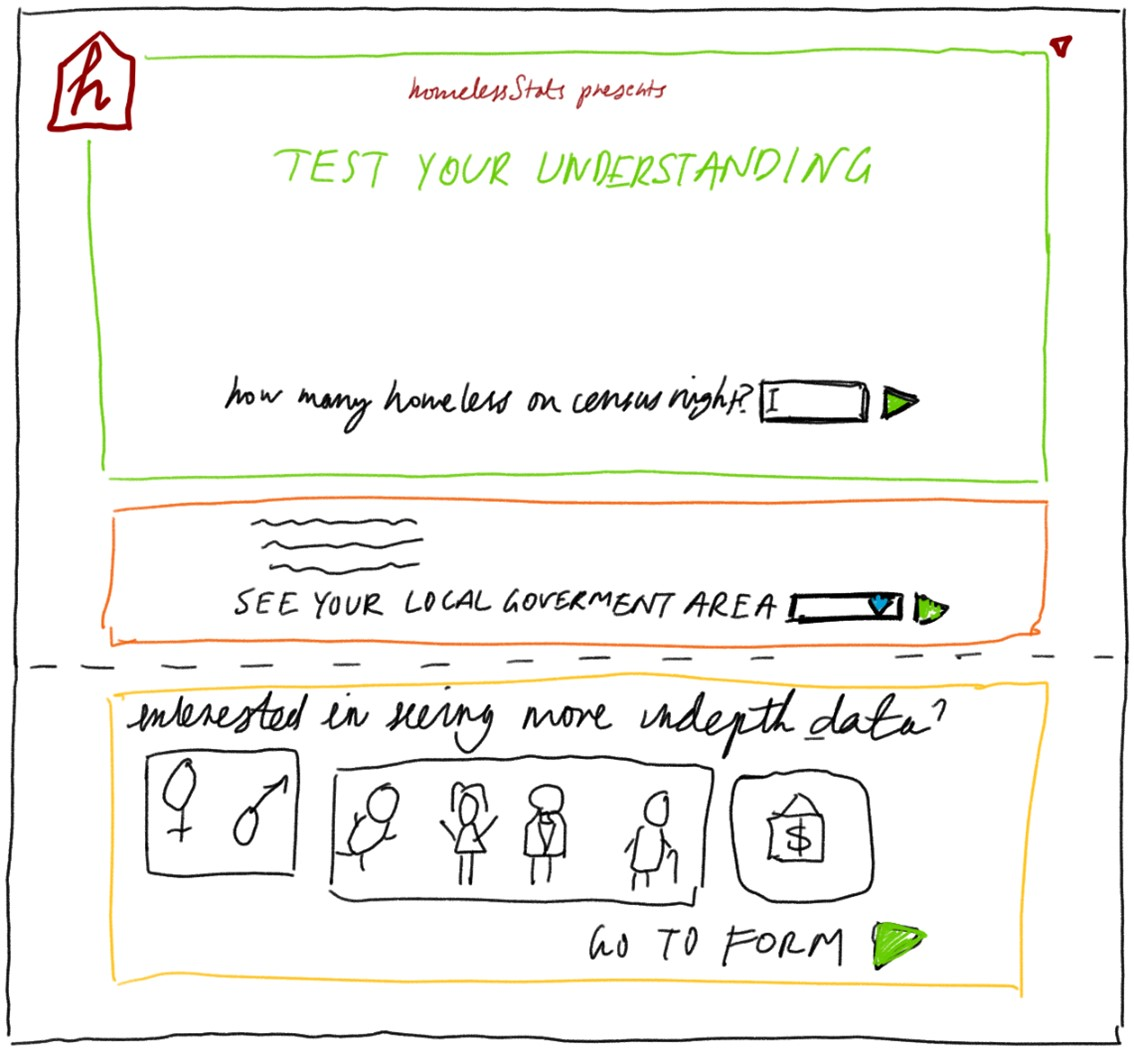
\includegraphics[scale=.8]{LandingPage.jpg} 
\caption{The landing page of the website}
\label{fig:erdiagram}
\end{figure}
The first feature, outlined in green, is a box that the user can click on to get through to the big picture page. Alternatively, the user can do the same thing in an interactive way by typing an answer into the text box to the question prompted and clicking on the arrow button. As Douglas’ goal is to learn more about homelessness, this allows him to test his understanding and facilitate his own learning.

The second feature, outlined in orange, is another box that users can click through to get to the shallow glance at homelessness page. It is populated with text that explains what data they will find on this page. A drop-down box following text that prompts the customer to choose their local government area and allows personalised results by clicking on the arrow button. This is especially helpful for Douglas, whose goal is to learn more about homelessness and how he can get involved, specifically in his own community.

The third feature, outlined in yellow, is another box that users can click through to go to fill out a form that then provides the user with a deeper dive into the data of homelessness. It has graphics to indicate what type of filters will be available to them in the form itself.

These boxes follow Neilson’s Consistency and Standards heuristic, allowing users to intuit that each box serves different functions. The arrows (coloured in green) align with Neilson’s Match Between System and the Real World heuristic, as it is commonly understood that arrows mean forward or to go, making users like Douglas who lack technical experience to use this feature. Identified as a strength in StreetSmart Australia’s website were the subtle call-to-actions at any point in the browsing experience, replicated in the arrows. Making our features consistent throughout the page minimises the user’s need to learn how to use the web page, as Neilson’s Recognition or Recall heuristic describes.
\subsection{Level 2}
\begin{figure}[h]
\centering
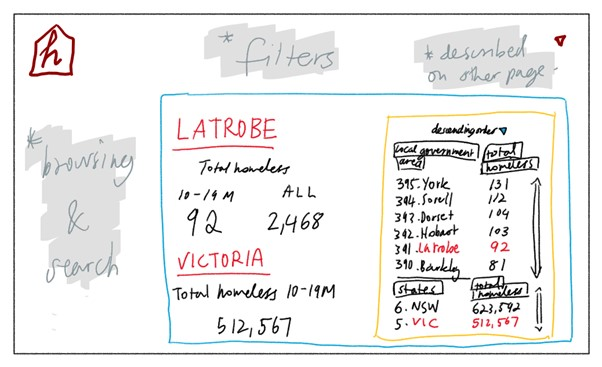
\includegraphics[scale=.8]{level2inner.jpg} 
\caption{The result section of the level two page}
\label{fig:erdiagram}
\end{figure}
The features that will be explained are those encased in the blue box, which form the result screen where users will see data and information, where the users have already chosen their search specifications.

The first feature, on the left side of the result box, will return the information they have searched for. By default, it provides all aggregated data of homeless people in Australia. If a state is selected, those details will populate. If an LGA is selected, it will appear at the top of the box and the corresponding state below.

The second feature, outlined in yellow, is a ranking table on the right of the result box. It corresponds with the filters chosen and the main information displayed on the left. Immediately, they can see how their LGA or state ranks in terms of total homeless numbers with filters applied. They can also choose to see the list in ascending or descending order.

The chosen local government area and/or state are highlighted through coloured text in the ranking table, meeting Neilson’s Visibility of System Status heuristic, where the user can receive feedback as they switch between different LGAs. The colour corresponds to other areas of the screen, meeting Neilson’s Consistency and Standards heuristic, in which the continuity allows users to easily find related information.

The ranking feature, separated to the side and is smaller compared to the main information table, presents information to users like Douglas, who is only seeking basic information about their community, while also being useful to Lisa, looking for comparative data for her assignment. This describes Neilson’s Flexibility and Efficiency of Use, where the basic user remains uninhibited while the more advanced user can draw some deeper insight.
\subsection{Level 3}
\begin{figure}[h]
\centering
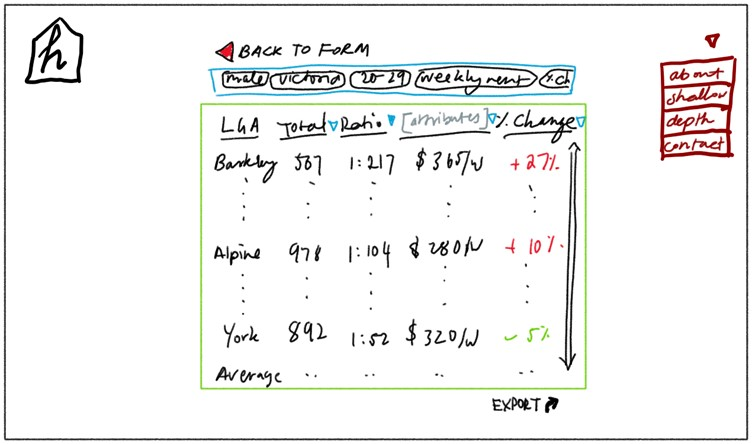
\includegraphics[scale=.8]{level3results.jpg} 
\caption{The results page of level 3}
\label{fig:erdiagram}
\end{figure}
This page serves to provide all the information that the user has requested in the form, in the form of a table.

The first feature is the results table, outlined in green. It is displayed in the middle of the page and expands outwards if more information has been requested in the form. It displays the LGA on the left as fixed and the table columns depend on user specification in the form page. The red button allows sorting in that column in ascending or descending order. It takes advantage of negative space to focus on the data the user has come for. Neilson’s Aesthetic and Minimalist design heuristic is displayed here through the absence any irrelevant information to increase the visibility of the table.

The specifications of the form are displayed in the second feature, outlined in blue. Having the options listed out in this way provides the user with Visibility of System Status, reminding them of the options that they have chosen and allows for review if required. This keeps them informed about exactly what they are seeing in the first feature.

The user can return to the form through the third feature, the back arrow, to edit their specifications to adjust the table. This provides the user with User Control and Freedom where Neilson describes allowing the user to quickly and simply return in case an error was made.

The table and the specifications can be exported for reference. Lisa, who is doing research on homelessness for her assignment, easily adjusts her preferences and is informed of her specifications until she is satisfied with the table of information and can export it for her own reference.

The user also has the option to return to the home page through the floating home button on the top left, at any point on the website, or navigate to other pages through the navigation drop down bar on the top right, extending on the User Control and Freedom heuristic.
\section{Database design}
It was necessary to design a database to allow our website to provide the information the user wants. A user must be able to make relational data queries such as 'show me the homeless ratio in LGA's that have a median weekly income lower than \$500'. We could have all of the information for the LGA's in the one table, with every attribute of that LGA in it's own column (eg. '2016\_homeless\_f\_0\_9' amount of female homeless people who are aged 0-9 in that LGA in 2016). With the current data we have, we would need 45 columns with that database design. 

A table with 45 columns is manageable and if we did not want this project to be scalable, this design would be fine. We want the database to grow as more research is conducted however, and we would be starting to add columns to our database if all the information was in one table. This would require the database to make a copy of the table with the new columns, transfer all of the previous entries and delete the original. The amount of columns in the table would also become more and more unmanageable as more research data becomes available. If we split the data up into multiple tables we avoid this issue and any new data is added as new data entries (rows) without having to do a complete restructure.

To decide how many entities (table) we needed and which attributes (columns) each entity should have, we analysed the data that we have and made an entity diagram (see figure \ref{fig:erdiagram}). The database modelled in the diagram allows for entry of new data without making new attributes. 

\begin{figure}[h]
\centering
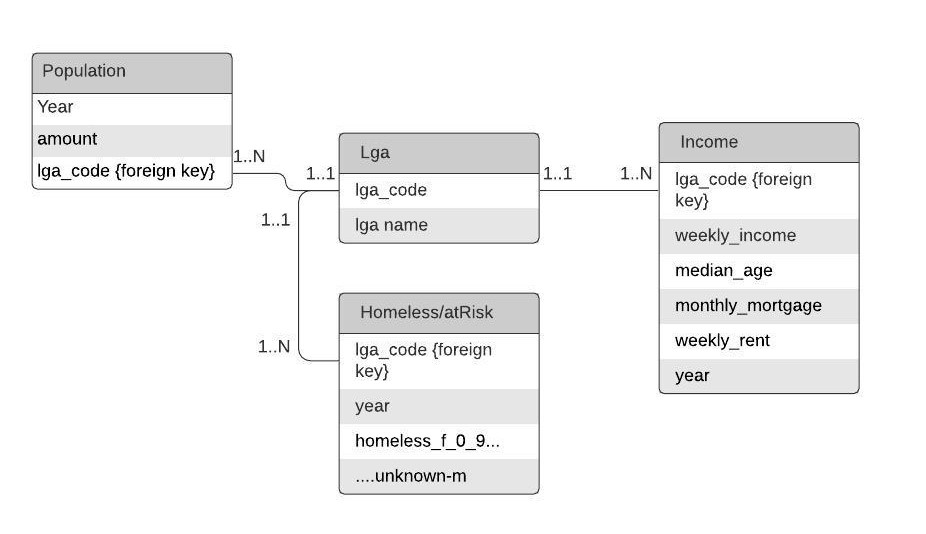
\includegraphics[scale=.8]{ERDiagram.jpg} 
\caption{Entity Relationship diagram of the diagram}
\label{fig:erdiagram}
\end{figure}

\textbf{Relational model}\\
A relational model can be extracted from this diagram:\\
Lga(\underline{lga\_code}, lga name)\\
Population(\underline{lga\_code*, year}, amount)\\
Income(\underline{lga\_code*, year}, weekly\_income, median\_age, monthly\_mortgage, weekly\_rent)\\
Homeless/AtRisk(\underline{lga\_code*, year}, **homeless\_f\_0\_9 ... unknown\_m )\\

\emph{**Note}: The Homeless/AtRisk entity has attributes between the ellipses. Each attribute is an integer amount of the people that meet the conditions stated. For example, the attribute 'homeless\_f\_0\_9' corresponds to people who are homeless, female and between the ages 0 and 9 inclusive. If this attribute were '7', the year attribute '2016' and the lga\_code was the code corresponding to Sunbury, it would mean there were 7 homeless female people aged 0-9 in 2016.\\

The database modelled in figure \ref{fig:erdiagram} enable the website to deliver any information that the user needs. As an example, lets look at how the database would work for a query. To illustrate it's capability we will choose a complex query:

\textbf{Query:} What is the ratio of homeless people against the total population in LGA's where the median weekly income is under \$500. We will assume the user wants the most recent data available and only use data from 2018
These are the steps that are needed in order to answer this query with the data that we have:
\begin{enumerate}
\item Find all of the LGA's that had a median weekly income under \$500 in 2018.
\item Calculate the total number of people in these LGA's who were homeless in 2018.
\item Find the total 2018 population of these LGA's.
\item Divide the result of step 2. by the result of step 3.
\end{enumerate}
In order to answer this query, our database would complete these steps:
\begin{enumerate}
\item Find all of the weekly\_income entries in the Income table that are less than 500 along with the corresponding LGA codes.
\item Find and sum the amounts of all homeless that correspond to these LGA codes in the Homeless/AtRisk table. (all of the attributes that begin with 'homeless' for each LGA.
\item Find and sum the amounts that corresponds to these codes and the year '2018' in the Population table.
\item Divide the result in step 2. by the result in step 3.
\end{enumerate} 

\textbf{Building the database:} \\
To build the database, we imported four csv files. Two files resembled two of the tables that we would need in the database: Population and Income. Another two files contained the information that we needed for our Homeless/AtRisk table. All of these files also contained the information needed to create the LGA table: LGA codes with corresponding LGA names. To build our database, we executed the following steps in Sqlite Studio:

\begin{enumerate}
\item Create a database and import all four csv files as tables using the GUI in Sqlite Studio. Resulting in tables: HRA2016, HRA2018, Population and Income.
\item Combine the 2016 and 2018 data on homeless people and people who are at risk of being homeless by executing: \\
\hspace*{10mm}%
INSERT INTO [HRA2018]\\
\hspace*{10mm}%
SELECT * FROM [HRA2016];\\
Then renaming HRA2018 to Homeless/AtRisk using the GUI.
\item Creating an LGA table and inserting the LGA code and name columns from the Income table (either Income or Population would have worked here):\\
\hspace*{10mm}%
CREATE TABLE [LGA](\\
\hspace*{10mm}%
lga\_code INT PRIMARY KEY NOT NULL,\\
\hspace*{10mm}%
lga\_name TEXT NOT NULL);\\
\hspace*{10mm}%
INSERT INTO [LGA]\\
\hspace*{10mm}%
SELECT lga\_code, lga\_name FROM Population;
\item Remove the column containing the LGA names from all tables excluding [LGA]. This can be done in a couple of ways, we chose to use the GUI.
\end{enumerate}
To test our database, we wrote SQL scripts corresponding to the queries that are available to the user. Our database will work in conjunction with Java to return the result: \\
\textbf{Query:} Show me how the rate of homelessness has changed between 2016 and 2018 in all LGA's compared to population.\\
A table with these three columns will be able to show the user this information: lga\_name, percentage change in the ratio of homeless people to the total population and the percentage change in population. To see the trend, the user can sort by the third column and then notice the change in numbers in the second column. The user can also easily see any net relationship by referring to the 'total' row at the top of the table, which will show a total change in the homeless ratio and the total change in population across the LGA's. \\
To produce this table, our database and Java will work in collaboration (in pseudocode):
\begin{enumerate}
\item Create a new table with the columns detailed above and insert lga\_names from the LGA table into the first column.
\item For each LGA (row), sum all of the columns that refer to homeless people in the Homeless/AtRisk table where the year = 2016.
\item Do the same where the year = 2018.
\item Divide result of 3. by the result of 2 and insert this result into column two of the created table.
\item Divide the 2018 and 2016 populations in the Population table and insert this into the third column.
\end{enumerate}
Each of the columns will match up with an LGA because all of the tables are sorted by lga\_code. \\
\textbf{Possible further database features}: \\
Currently we are unsure how we are going to save the level 3 form data for when the user wants to change their query. It may be that we can use html for this but we might have to create a table in the database that stores information on what the user selected in the form. There would be a column for each possible value of every input the user selects. \\

\section{References}
Nielsen, Jakob, and Rolf Molich. “Heuristic Evaluation of User Interfaces.” Proceedings of the SIGCHI Conference on Human Factors in Computing Systems. ACM, 1990. 249–256. Web. \\


\end{document}
